\section{Volumes}
\subsection{Volumes from Cross Sections}
Imagine we want to find the volume of some complex object.
One way we could approximate it is by slicing it into narrow cross sections.
The volume of each cross section would roughly be the area of the cross sectional face, times the width of the cross section.

\begin{figure}[H]
	\label{volumes}
	\centering
	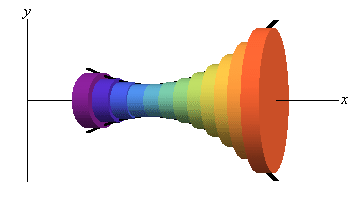
\includegraphics[width=0.5\textwidth]{./applications_integrals/volumes.png}
	\caption{\hyperref{https://tutorial.math.lamar.edu/classes/calci/Area\_Volume\_Formulas.aspx}{}{}{Paul's Online Notes - Area and Volume Formulas}}
\end{figure}

Adding the volumes of these cross sections up, we'd get our approximation, which would get better and better the narrower the width of each cross section.
In the limit, this is exactly the definition of an integral.

\begin{definition}
	The volume of a solid with integrable corss sectional area $A(x)$ from $x=a$ to $x=b$ is given by
	\begin{equation*}
		V = \int_{a}^{b}{A(x)\d{x}}.
	\end{equation*}
\end{definition}


Let's start by finding the volume of a solid we already know.
\begin{example}
	Find the volume of a cube with sidelength $a$.
\end{example}
\begin{answer}
	For any slice of a cube, the cross section is a square with sidelength $a$.
	\begin{align*}
		A(x) &= a^2 \\
		V &= \int_{0}^{a}{a^2\d{x}} \\
		&= a^2x\biggr\rvert_0^a \\
		&= a^3.
	\end{align*}
\end{answer}


Now let's find the volume of a slightly more complicated shape.
\begin{example}
	Find the volume of a square pyramid with base sidelength $a$ and height $h$.
\end{example}
\begin{answer}
	Like the cube, any slice of the square pyramid is a square.
	However, the sidelength of the square depends on the height of your slice.
	A slice at the very tip of the pyramid would have sidelength 0, while a slice at the very bottom of the pyramid would have sidelength $a$.
	The sidelength grows linearly from $x=0$ to $x=h$, so it must be $\frac{a}{h}x$.
	\begin{align*}
		A(x) &= \left(\frac{a}{h}x\right)^2 \\
		V &= \int_{0}^{h}{\frac{a^2}{h^2}x^2\d{x}} \\
		&= \frac{a^2}{3h^2}x^3 \biggr\rvert_0^h \\
		&= \frac{a^2h}{3} \\
		&= \frac{1}{3}a^2 h.
	\end{align*}
\end{answer}

\subsection{Solids of Revolution}
You can think of solids of revolution as a special case of volumes from cross sections.
We'll tend to be on the lookout for a function that defines the radius, and we can then use the formula for the area of a circle to get the cross sectional area.
\begin{equation*}
	A(x) = \pi r^2(x).
\end{equation*}

\begin{example}
	Find the volume of the cone formed by rotating the line $y=x/3$ about the $x$-axis for $0 \leq x \leq 6$.
\end{example}
\begin{answer}
	The radius is simply the distance from the $x$-axis, which is just another name for $y$.
	So,
	\begin{equation*}
		A(x) = \pi \left(\frac{x}{3}\right)^2.
	\end{equation*}
	
	Integrating,
	\begin{align*}
		V &= \int_{0}^{6}{\pi\left(\frac{x}{3}\right)^2\d{x}} \\
		&= \frac{\pi}{9}\int_{0}^{6}{x^2\d{x}} \\
		&= \frac{\pi}{9}\left(\frac{x^3}{3}\biggr\rvert_0^6\right) \\
		&= 8\pi.
	\end{align*}
	
	This is the volume of a cone with radius 2 and height 6: $\frac{1}{3}\pi(2)^2(6)=8\pi$.
\end{answer}


Let's try a more complicated solid.
\begin{example}
	Find the volume of the solid of revolution bounded by $y=2+x\cos{x}$ from $-\frac{\pi}{2} \leq x \leq \frac{\pi}{2}$.
\end{example}
\begin{answer}
	Again, the radius is simply the distance from the $x$-axis, which is $y$.
	\begin{align*}
		A(x) &= \pi \left(2+x\cos{x}\right)^2 \\
		&= \pi \left(4 + 4x\cos{x} + x^2\cos^2{x}\right) \\
		V &= \int_{-\pi/2}^{\pi/2}{\pi \left(4 + 4x\cos{x} + x^2\cos^2{x}\right)\d{x}} \\
		&= \pi\left(\int_{-\pi/2}^{\pi/2}{4\d{x}}+\int_{-\pi/2}^{\pi/2}{4x\cos{x}\d{x}}+\int_{-\pi/2}^{\pi/2}{x^2\cos^2{x}\d{x}}\right) \\
		&= \pi\left(4\pi + 0 + \frac{1}{24}\pi\left(\pi^2-6\right)\right) \text{ (use integration by parts)}\\
		&= \frac{\pi^4}{24} + \frac{15\pi^2}{4}.
	\end{align*}
\end{answer}

\subsubsection{Washer Method}
Imagine now we want to find the volume of a solid of revolution with a ``hole.``
''If we were to take a cross section of such a solid, it'd look like a washer with an outer radius $R(x)$ and inner radius $r(x)$.

\begin{figure}[H]
	\label{washers}
	\centering
	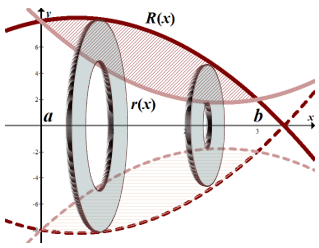
\includegraphics[width=0.33\textwidth]{./applications_integrals/Washer-1.png}
	\caption{\hyperref{https://www.shelovesmath.com/calculus/integral-calculus/applications-integration-area-volume/}{}{}{She Loves Math - Applications of Integration: Area and Volume}}
\end{figure}


We can think of this in a similar way as the area between curves in 2D.
We'll find the volume swept by the outer radius and the subtract the volume swept and removed by the inner radius.
\begin{equation*}
	V = \pi\int_{a}^{b}{(R^2(x)-r^2(x))\d{x}}.
\end{equation*}

\begin{example}
	Find the volume of shape formed by revolving the area enclosed by the $y$-axis, $y=\cos{x}$, and $y=\sin{x}$ around the $x$-axis.
\end{example}
\begin{answer}
	In the first quadrant, $\cos{x} \geq \sin{x}$ for $x \leq \frac{\pi}{4}$, so our bounds are $0 \leq x \leq \frac{\pi}{4}$, $R(x)=\cos{x}$, and $r(x)=\sin{x}$.
	\begin{align*}
		V &= \pi\int_{0}^{\pi/4}{(\cos^2{x}-\sin^2{x})\d{x}} \\
		&= \pi\int_{0}^{\pi/4}{\cos{(2x)}\d{x}} \\
		&= \pi\left(\frac{\sin{2x}}{2}\right)\biggr\rvert_0^{\pi/4} \\
		&= \frac{\pi}{2}.
	\end{align*}
\end{answer}

\subsubsection{Cylindrical Shells Method}
All the previous methods for finding the volumes of solids of rotation have relied on summing the volumes of thin cross sectional slices that are perpendicular to the axis of rotation.
However, we can instead sum the volume of thin cylindrical shells that grow outwards from and parallel to the axis of revolution.

\begin{figure}[H]
	\label{shells}
	\centering
	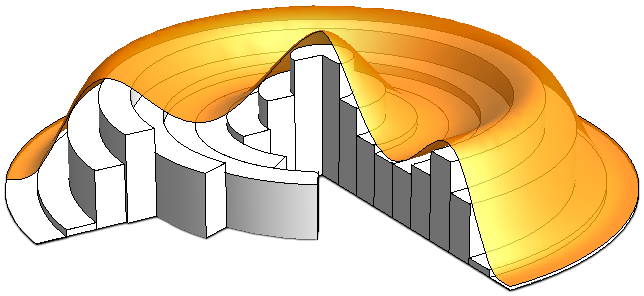
\includegraphics[width=0.5\textwidth]{./applications_integrals/shells.png}
	\caption{\hyperref{https://en.wikipedia.org/wiki/Shell\_integration}{}{}{Wikipedia - Shell Integration}}
\end{figure}


Each cylindrical shell will have a radius $r(x)$, a height $h(x)$, and a thickness $\d{x}$, meaning a volume of $2\pi r(x)h(x)\d{x}$.
\begin{equation*}
	V = 2\pi\int_{a}^{b}{r(x)h(x)\d{x}}.
\end{equation*}

\begin{example}
	Find the volume of the area bounded by the $y$-axis, $y=4-x^2$, and $y=x$ revolved around the $y$-axis.
\end{example}
\begin{answer}
	Each shell's height is parallel to the axis of rotation.
	In this case that's the distance between the two curves.
	\begin{equation*}
		h(x) = 4-x^2-x \text{ and } r(x)=x.
	\end{equation*}
	
	The two curves intersect at $x=\frac{-1+\sqrt{17}}{2}$.
	Finding the volume,
	\begin{align*}
		V &= 2\pi\int_{0}^{\frac{-1+\sqrt{17}}{2}}{x(4-x^2-x)\d{x}} \\
		&= 2\pi\left(-\frac{x^4}{4}-\frac{x^3}{3}+2x^2\right)\biggr\rvert_{0}^{\frac{-1+\sqrt{17}}{2}} \\
		&= \frac{\pi}{12}\left(121-17\sqrt{17}\right).
	\end{align*}
\end{answer}

\begin{example}
	Find the volume of the area bounded by the $x$-axis and the curve $y=(x-1)^2(x-2)^2$ rotated about the $y$-axis.
\end{example}
\begin{answer}
	The height of the shell is parallel to the $y$-axis.
	In this case it's exactly equal to the value of the bounding curve.
	\begin{equation*}
		h(x)=(x-1)^2(x-2)^2 \text{ and } r(x)=x.
	\end{equation*}
	
	Finding the volume,
	\begin{align*}
		V &= 2\pi\int_{1}^{2}{x(x-1)^2(x-2)^2\d{x}} \\
		&= 2\pi\left(\frac{x^6}{6}-\frac{6x^5}{5}+\frac{13x^4}{4}-4x^3+2x^2\right)\biggr\rvert_{1}^{2} \\
		&= \frac{\pi}{10}.
	\end{align*}
\end{answer}

\subsubsection{Other Axes of Rotation}
Although rotating about the $x$ and $y$ axes are the most common, the methods we have here apply to rotating about any axis parallel to the $x$ or $y$ axis.
The includes any lines of the form $y=k$ or $x=k$ where $k$ is some constant. \\


One valid approach is simply to rewrite the equations for your bounding curves by shifting them such that your axis of rotation is the $x$ or $y$ axis.
However, it's often more convenient to not rewrite the equations and simply apply the methods.

\begin{example}
	Find the volume of the solid generated by rotating the region in the first quadrant bounded by $y=x^2$ and $y=2x$ about the line $x=-2$.
\end{example}
\begin{answer}
	We can use the washer method (although shells also works).
	Since we're rotating about a line parallel to the $y$-axis, we'll have to rewrite our equations in the form $x=\ldots$.
	\begin{equation*}
		x = \sqrt{y} \text{ and } x = \frac{y}{2}.
	\end{equation*}
	
	The inner radius is given by the distance from $x=-2$ to $x=y/2$, and the outer radius is given by the distance from $x=-2$ to $x=\sqrt{y}$.
	The curves intersect at $y=0$ and $y=4$.
	\begin{align*}
		r(x) = 2 + \frac{y}{2} &\text{ and } R(x) = 2 + \sqrt{y} \\
		V &= \pi\int_{0}^{4}{(2+\sqrt{y})^2-\left(2+\frac{y}{2}\right)^2\d{y}} \\
		&= \pi\int_{0}^{4}{\left(4\sqrt{y}-y-\frac{y^2}{4}\right)\d{y}} \\
		&= 8\pi.
	\end{align*}
\end{answer}

\begin{example}
	Find the volume of the solid generated by rotating the region bounded by $y=x^2$ and $y=x+2$ about the line $x=3$.
\end{example} 
\begin{answer}
	We can use the shells method.
	Our height is simply the difference in $y$ values between the two curves.
	The radius is the distance between the lines $x=3$ and $x+2$.
	\begin{equation*}
		h(x) = x+2-x^2 \text{ and } r(x) = 3-x.
	\end{equation*}
	
	The curves intersect at $x=-1$ and $x=2$.
	Finding the volume,
	\begin{align*}
		V &= 2\pi\int_{-1}^{2}{(3-x)(x+2-x^2)\d{x}} \\
		&= 2\pi\left(\frac{x^4}{4}-\frac{4x^3}{3}+\frac{x^2}{2}+6x\right)\biggr\rvert_{-1}^{2} \\
		&= \frac{45\pi}{2}.
	\end{align*}
\end{answer}

\subsubsection{Surface Area}
Can apply the idea behind shell integration to derive a formula for surface area of a solid of rotation.
A cylindrical shell would have height $\d{s}$, which is given to us by the arc length formula, and radius $x$ or $y$, if the axis of rotation is the $y$ or $x$ axis respectively.
\begin{align*}
	S &= \begin{cases}
		2\pi\int{y\d{s}} & \text{Rotation about $x$-axis} \\
		2\pi\int{x\d{x}} & \text{Rotation about the $y$-axis}
	\end{cases} \\
	& \text{where } \\
	\d{s} &= \begin{cases}
		\sqrt{1+\left(\dd{y}{x}\right)^2}\d{x} & y=f(x) \\
		\sqrt{1+\left(\dd{x}{y}\right)^2}\d{y} & x=g(y) \\
	\end{cases}.
\end{align*}

\begin{example}
	Find the surface area of a sphere with radius $r$.
\end{example}
\begin{answer}
	We can obtain a sphere by rotating $y=\sqrt{r^2-x^2}, -r\leq x\leq r$ about the $x$-axis.
	\begin{align*}
		\dd{y}{x} &= \frac{-x}{\sqrt{r^2-x^2}} \\
		\left(\dd{y}{x}\right)^2 &= \frac{x^2}{r^2-x^2} \\
		S &= 2\pi\int_{-r}^{r}{y\sqrt{1+\frac{x^2}{r^2-x^2}}\d{x}} \\
		&= 2\pi\int_{-r}^{r}{\sqrt{r^2-x^2}\frac{r}{\sqrt{r^2-x^2}}\d{x}} \\
		&= 2\pi\int_{-r}^{r}{r\d{x}} \\
		&= 4\pi r^2.
	\end{align*}
\end{answer}